\documentclass[journal]{IEEEtran}

\usepackage[T1]{fontenc}% optional T1 font encoding

\usepackage[pdftex]{graphicx}

\ifCLASSOPTIONcompsoc
\usepackage[caption=false,font=normalsize,labelfon
t=sf,textfont=sf]{subfig}
\else
\usepackage[caption=false,font=footnotesize]{subfi
g}
\fi

\begin{document}

\begin{figure*}
\centering
\subfloat[Target reconstruction with 256 acquisitions]{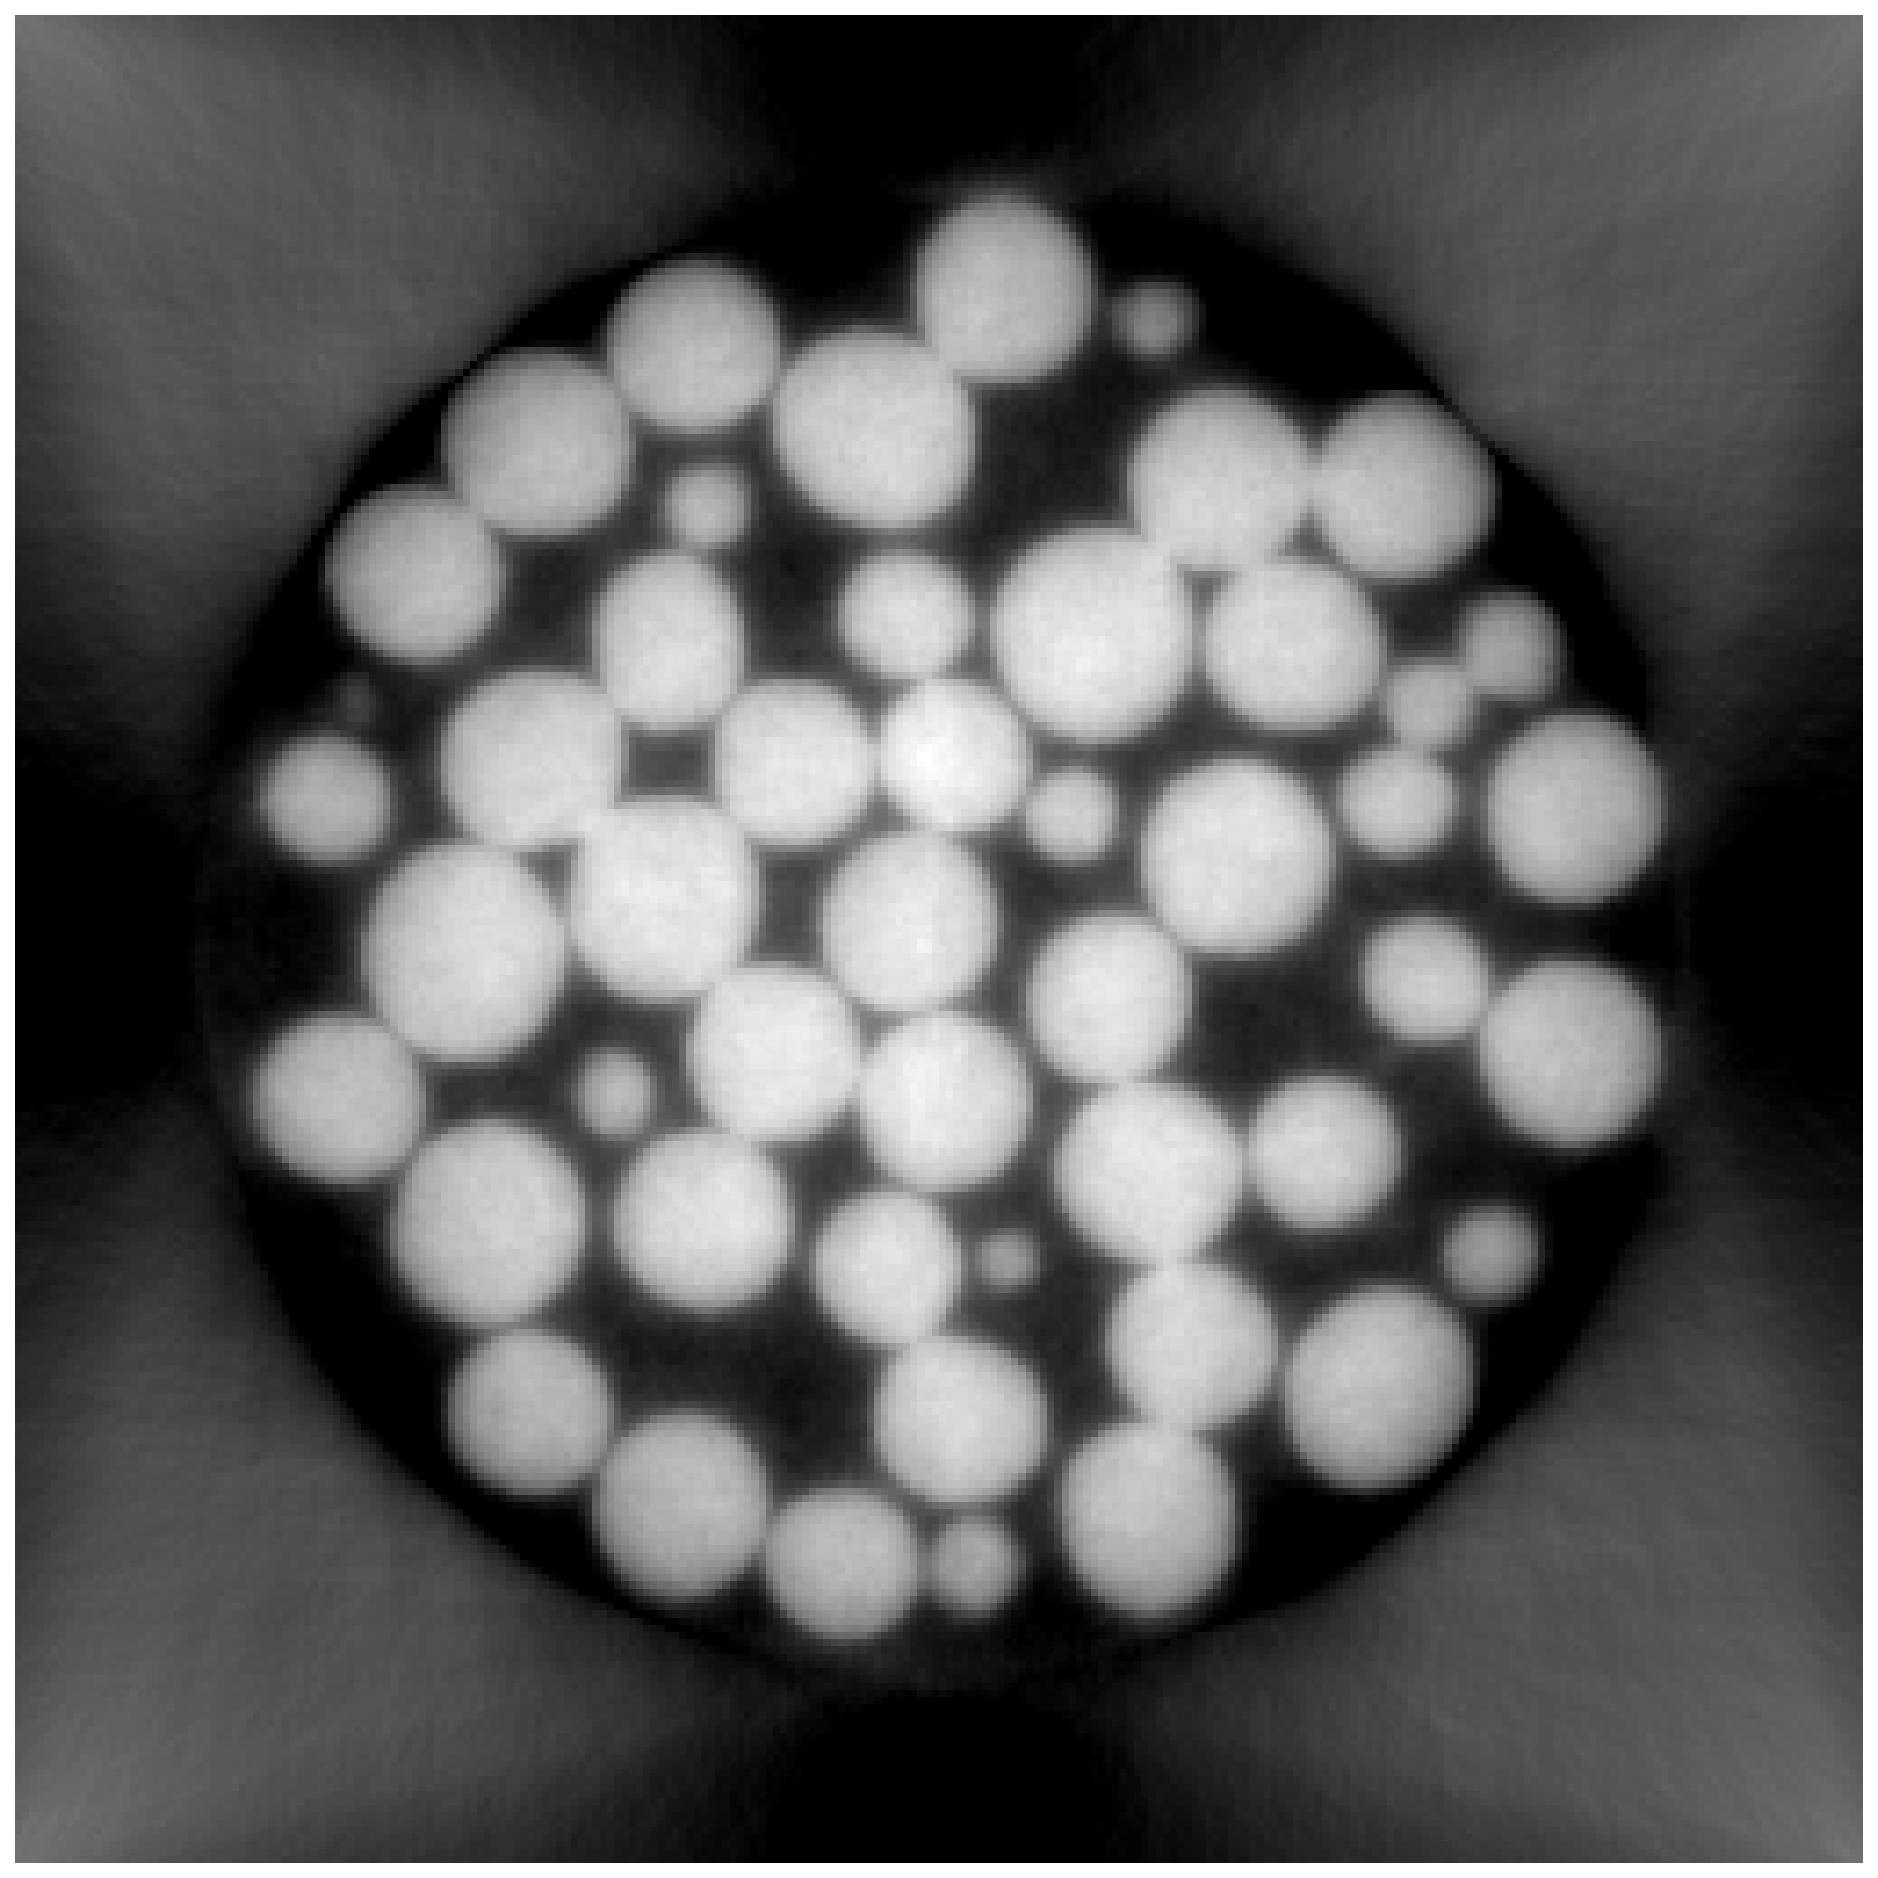
\includegraphics[width=0.2\textwidth]{ reconstructions128_target.jpg}
\label{fig:reconstructions128_target}}
\hfill
\subfloat[Reconstruction without any interpolation method , i.e from 128 acquisitions]{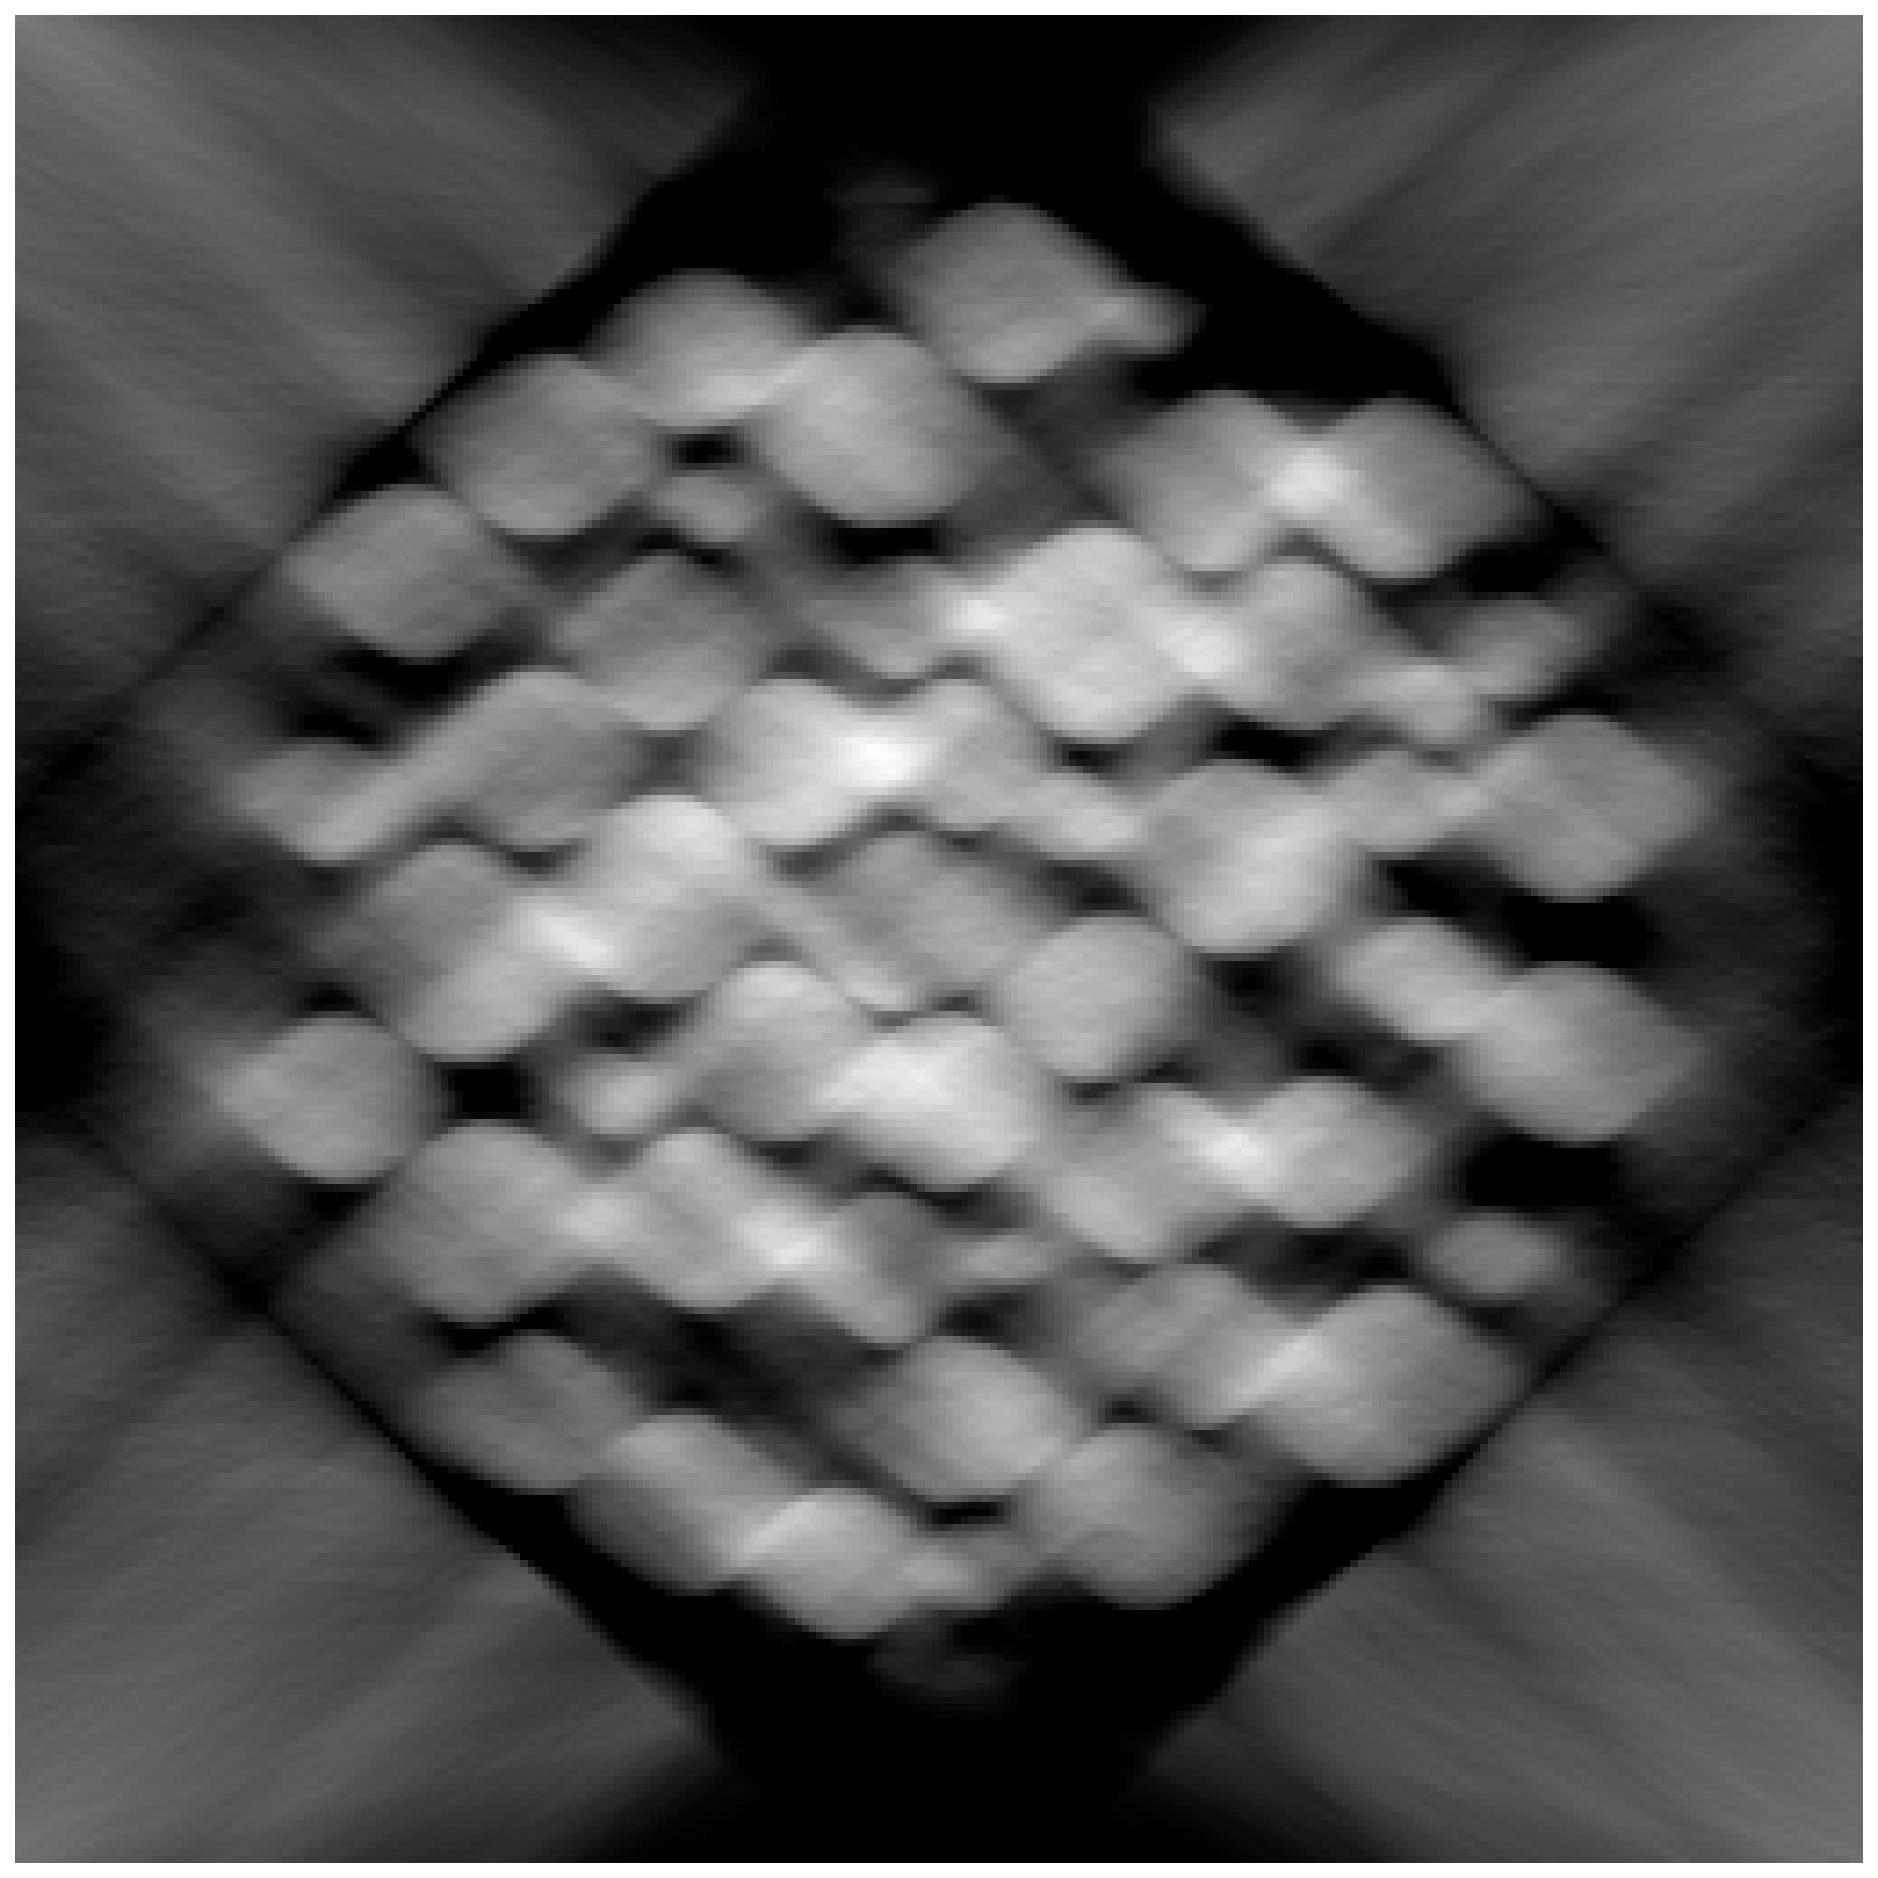
\includegraphics[width=0.2\textwidth]{ reconstructions128_noInterpolation.jpg}
\label{fig:reconstructions128_noInterpolation}}
\hfill
\subfloat[Reconstruction with linear interpolation]{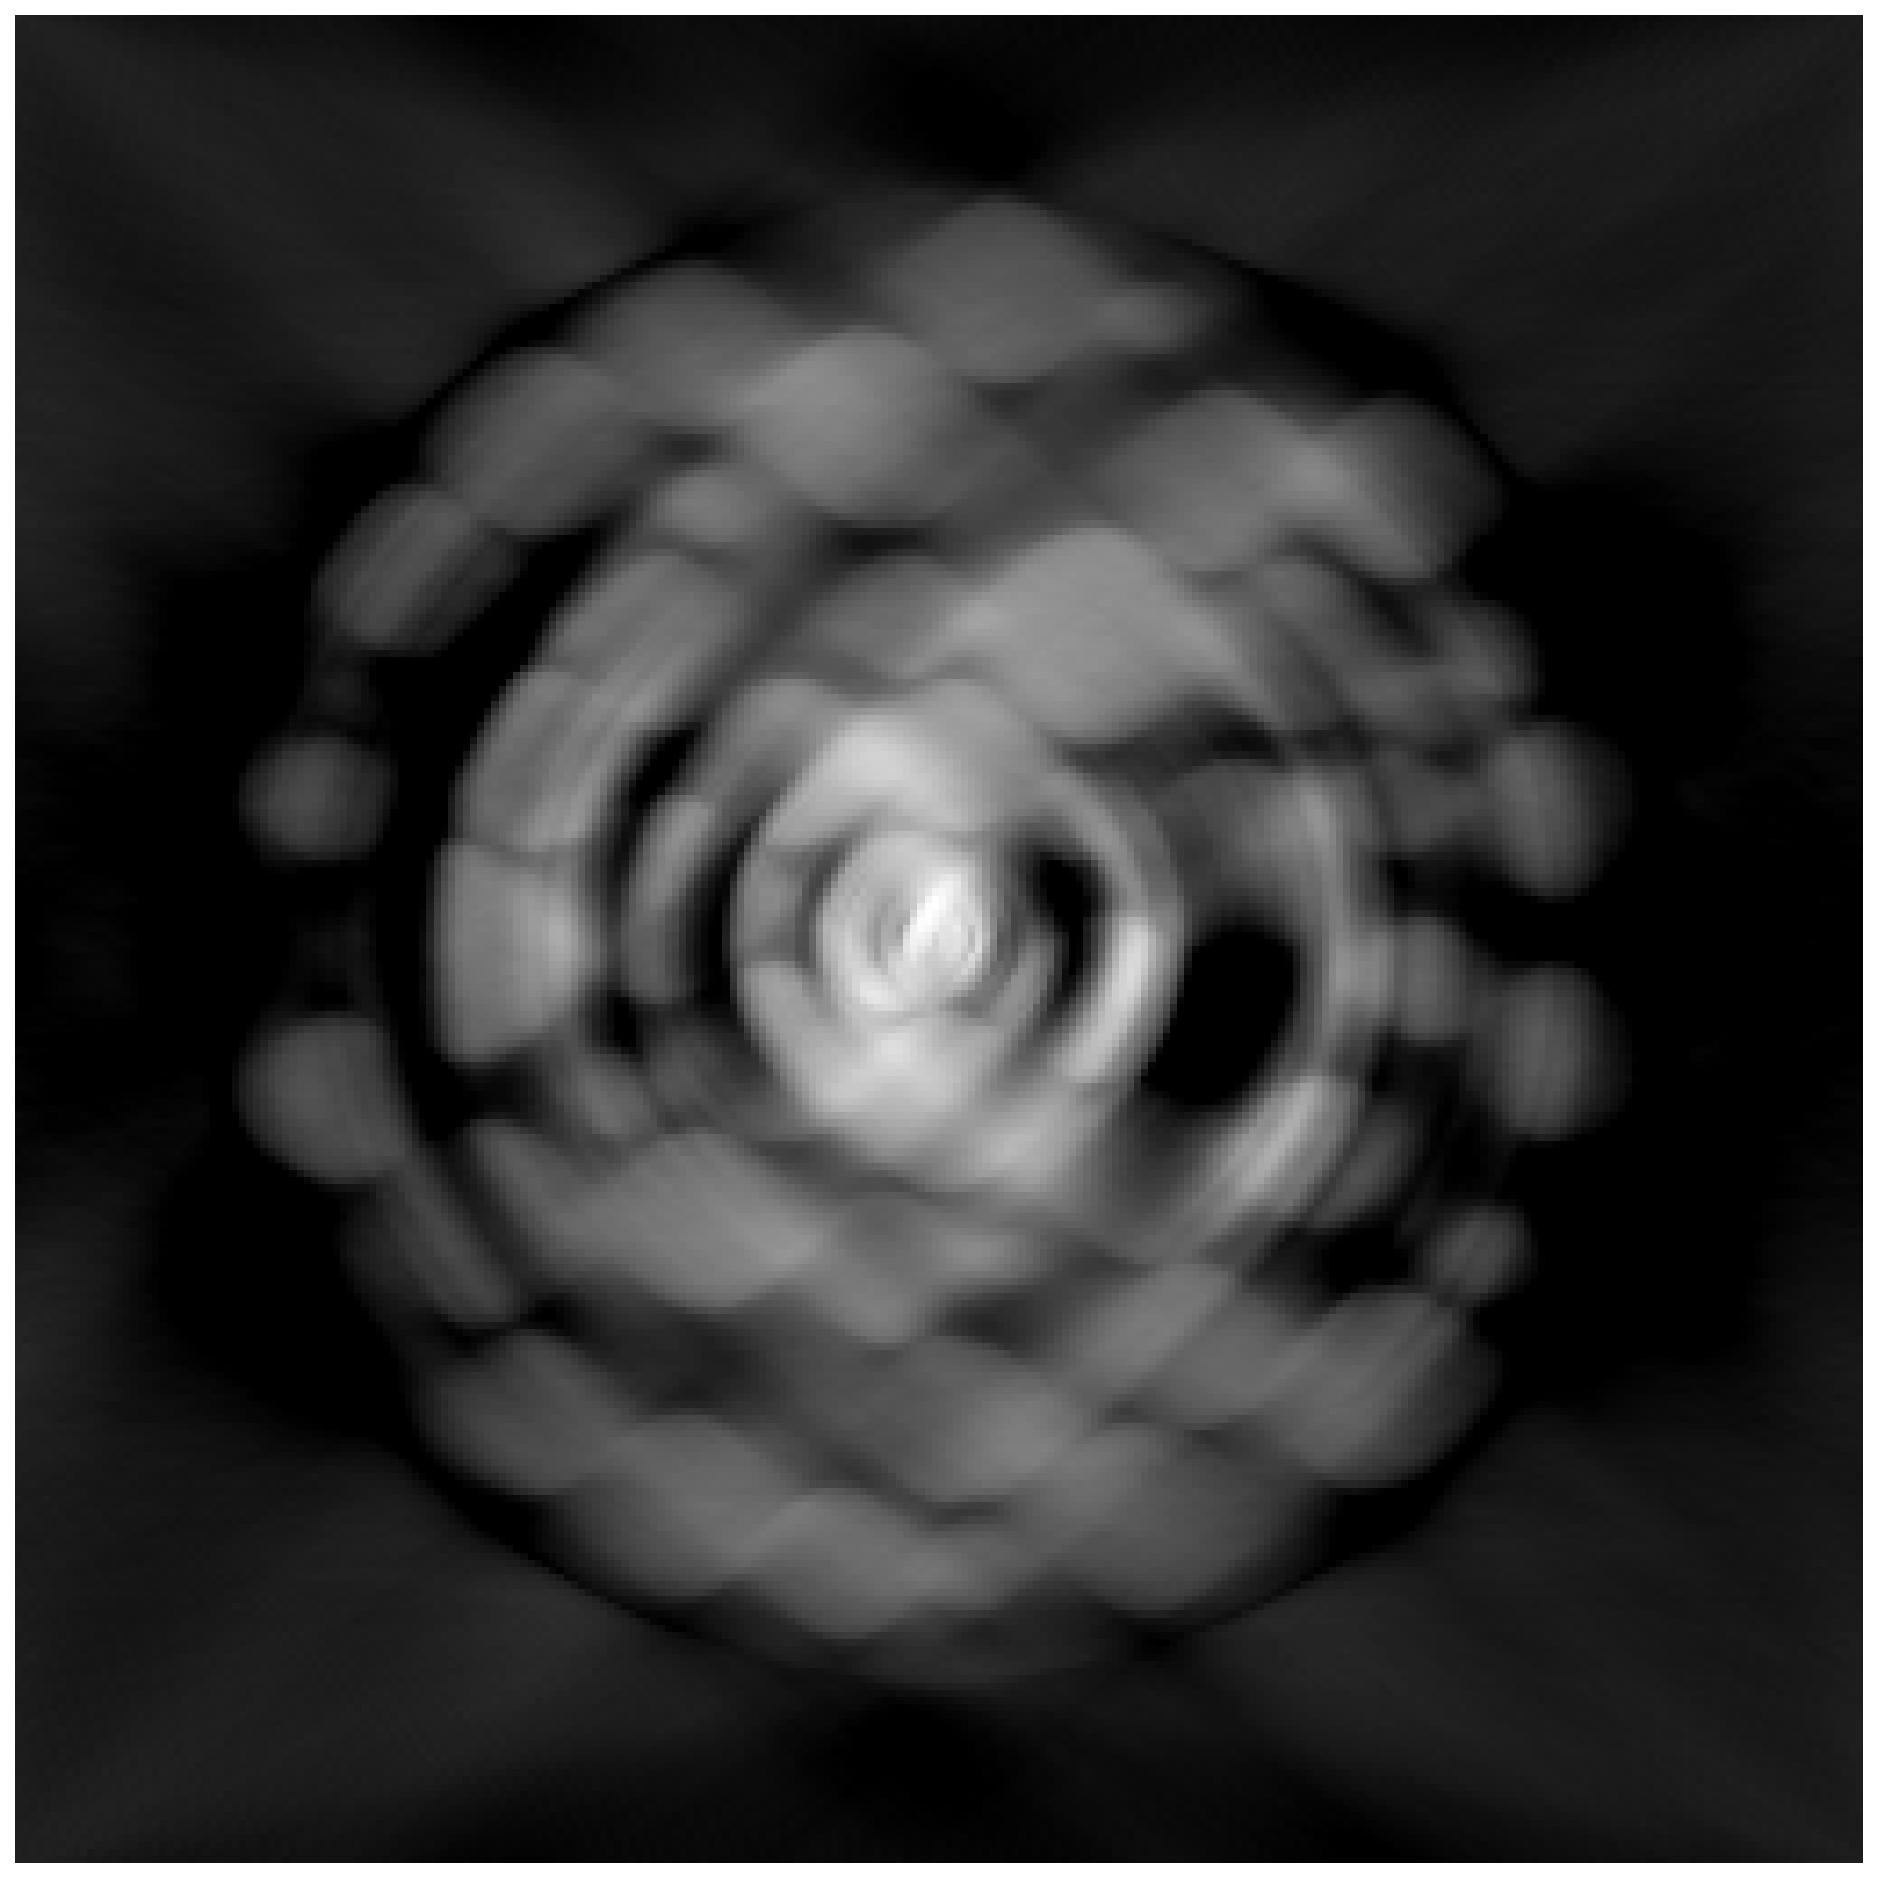
\includegraphics[width=0.2\textwidth]{ reconstructions128_linearInterpolation.jpg}
\label{fig:reconstructions128_linearInterpolation}}
\hfill
\subfloat[Reconstruction with missing acquisitions replaced by CAD-expected ones]{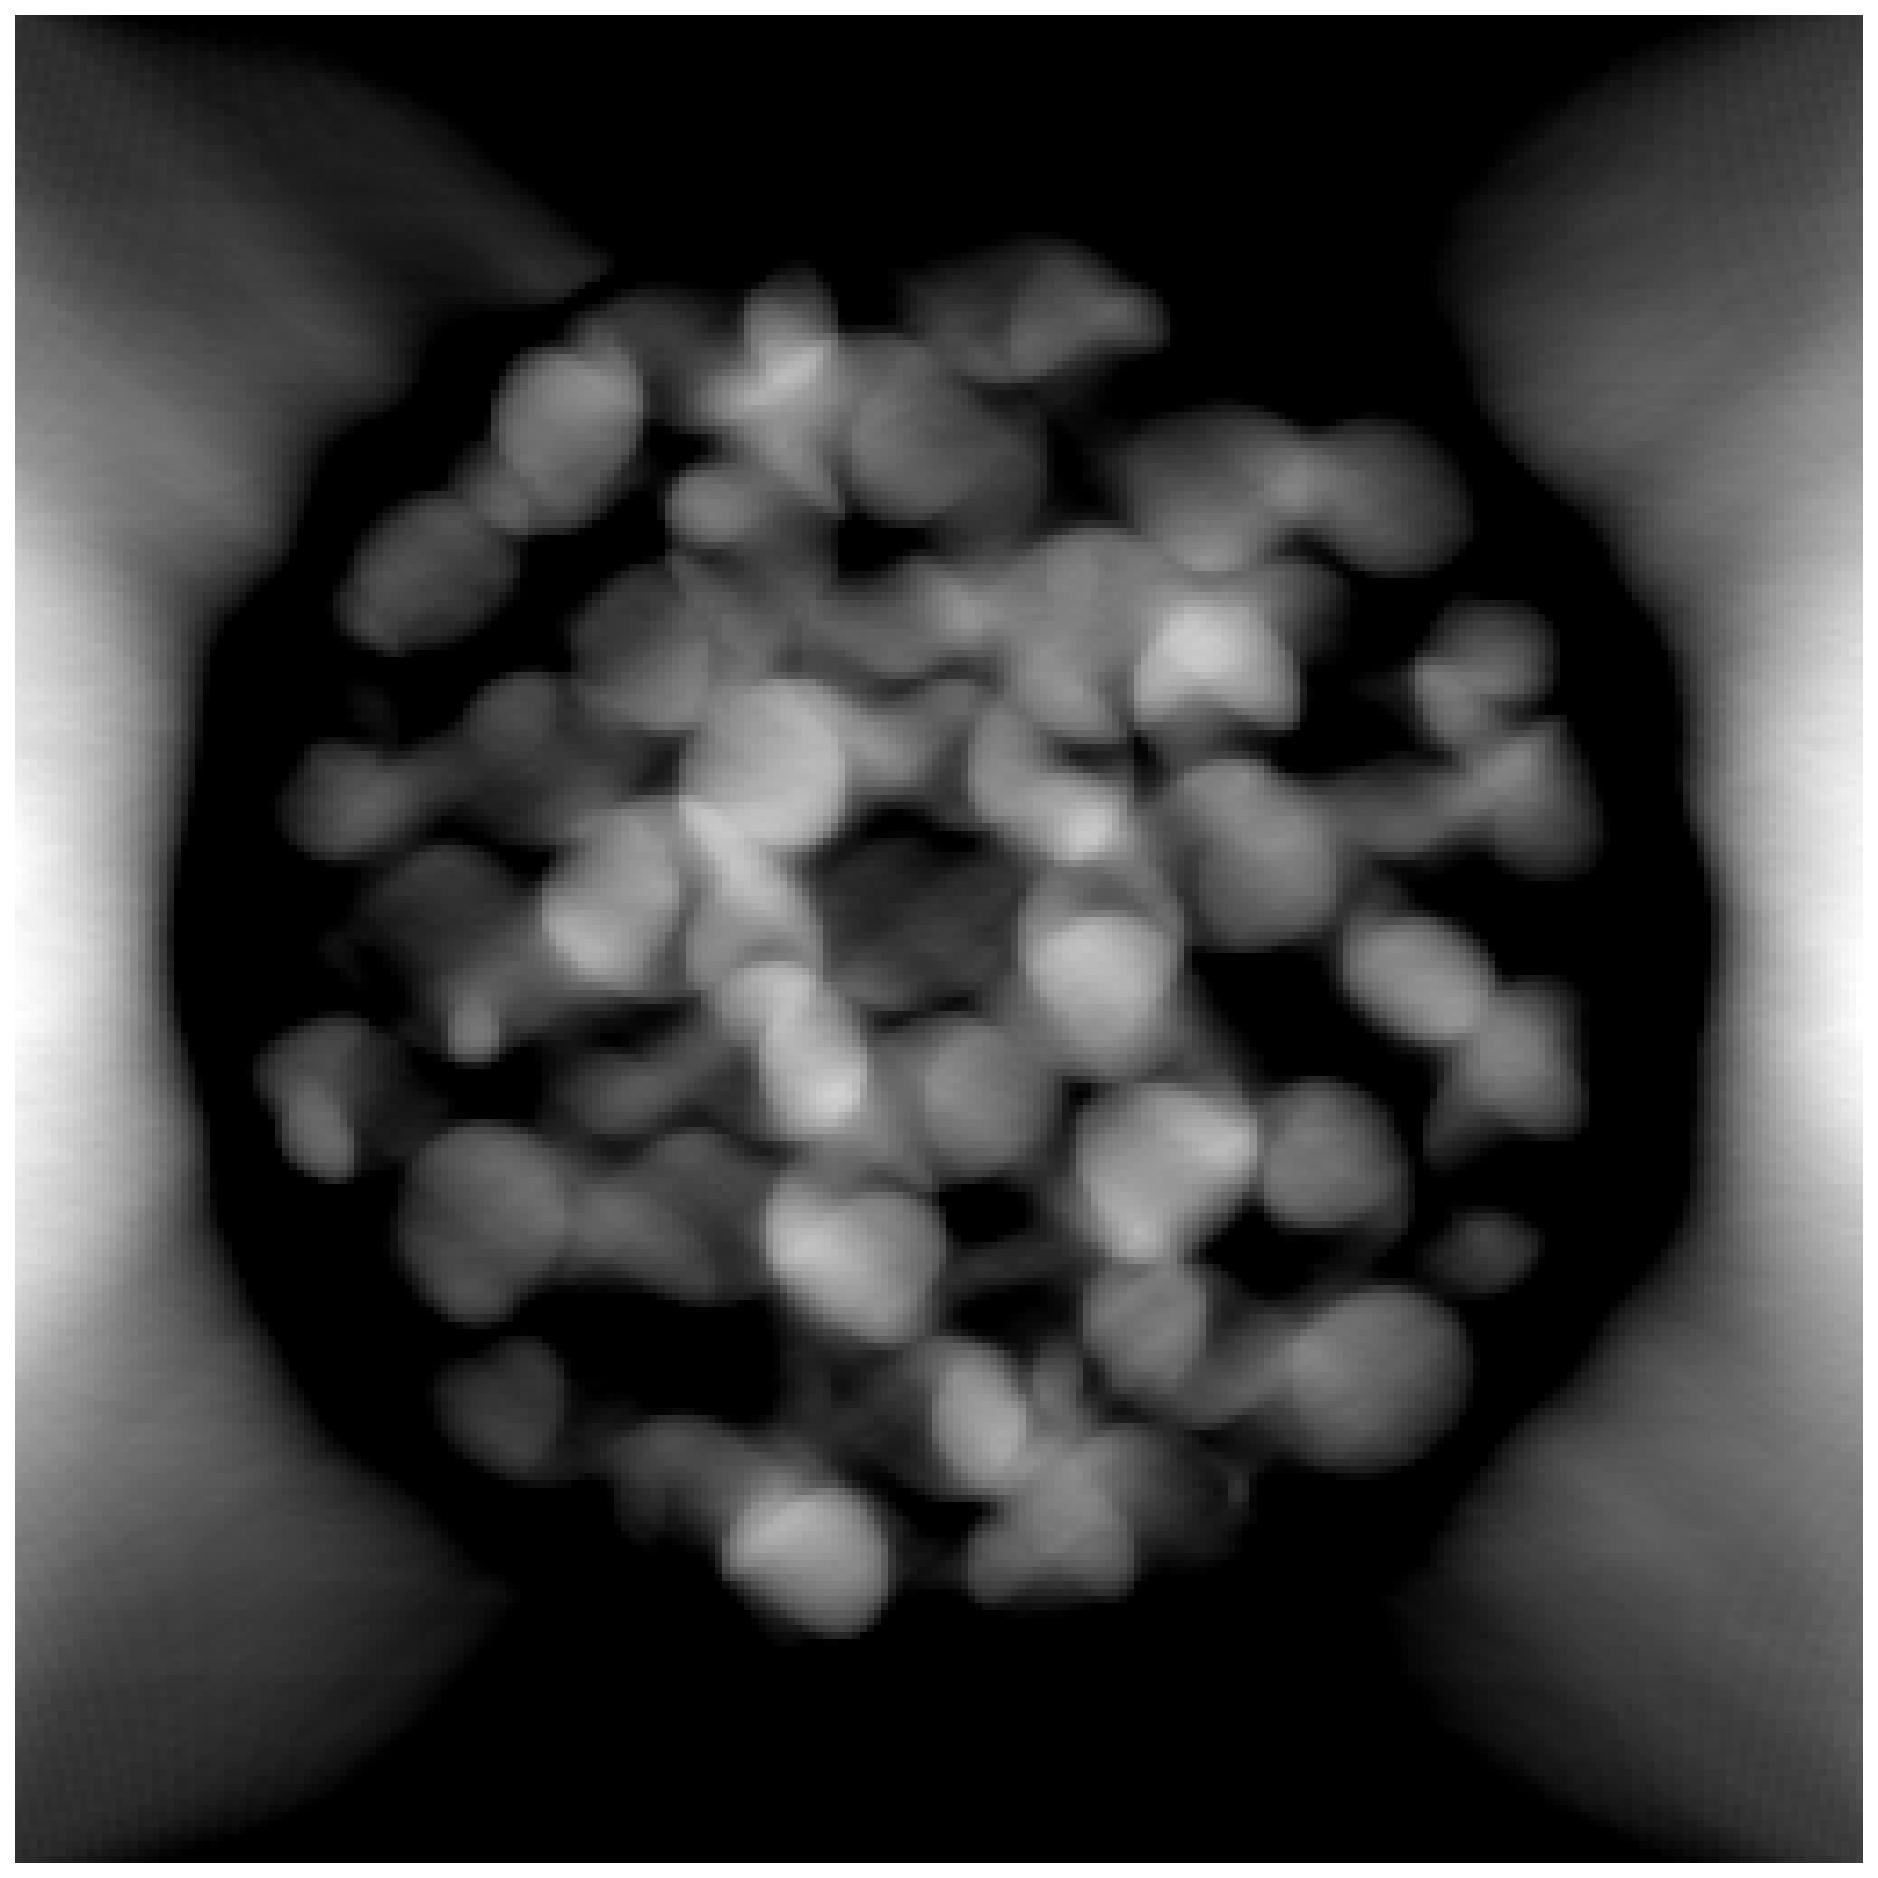
\includegraphics[width=0.2\textwidth]{ reconstructions128_inferenceCad.jpg}
\label{fig:reconstructions128_inferenceCad}}
\hfill
\subfloat[Reconstruction with acquisitions inferred from the Unet without the CAD prior]{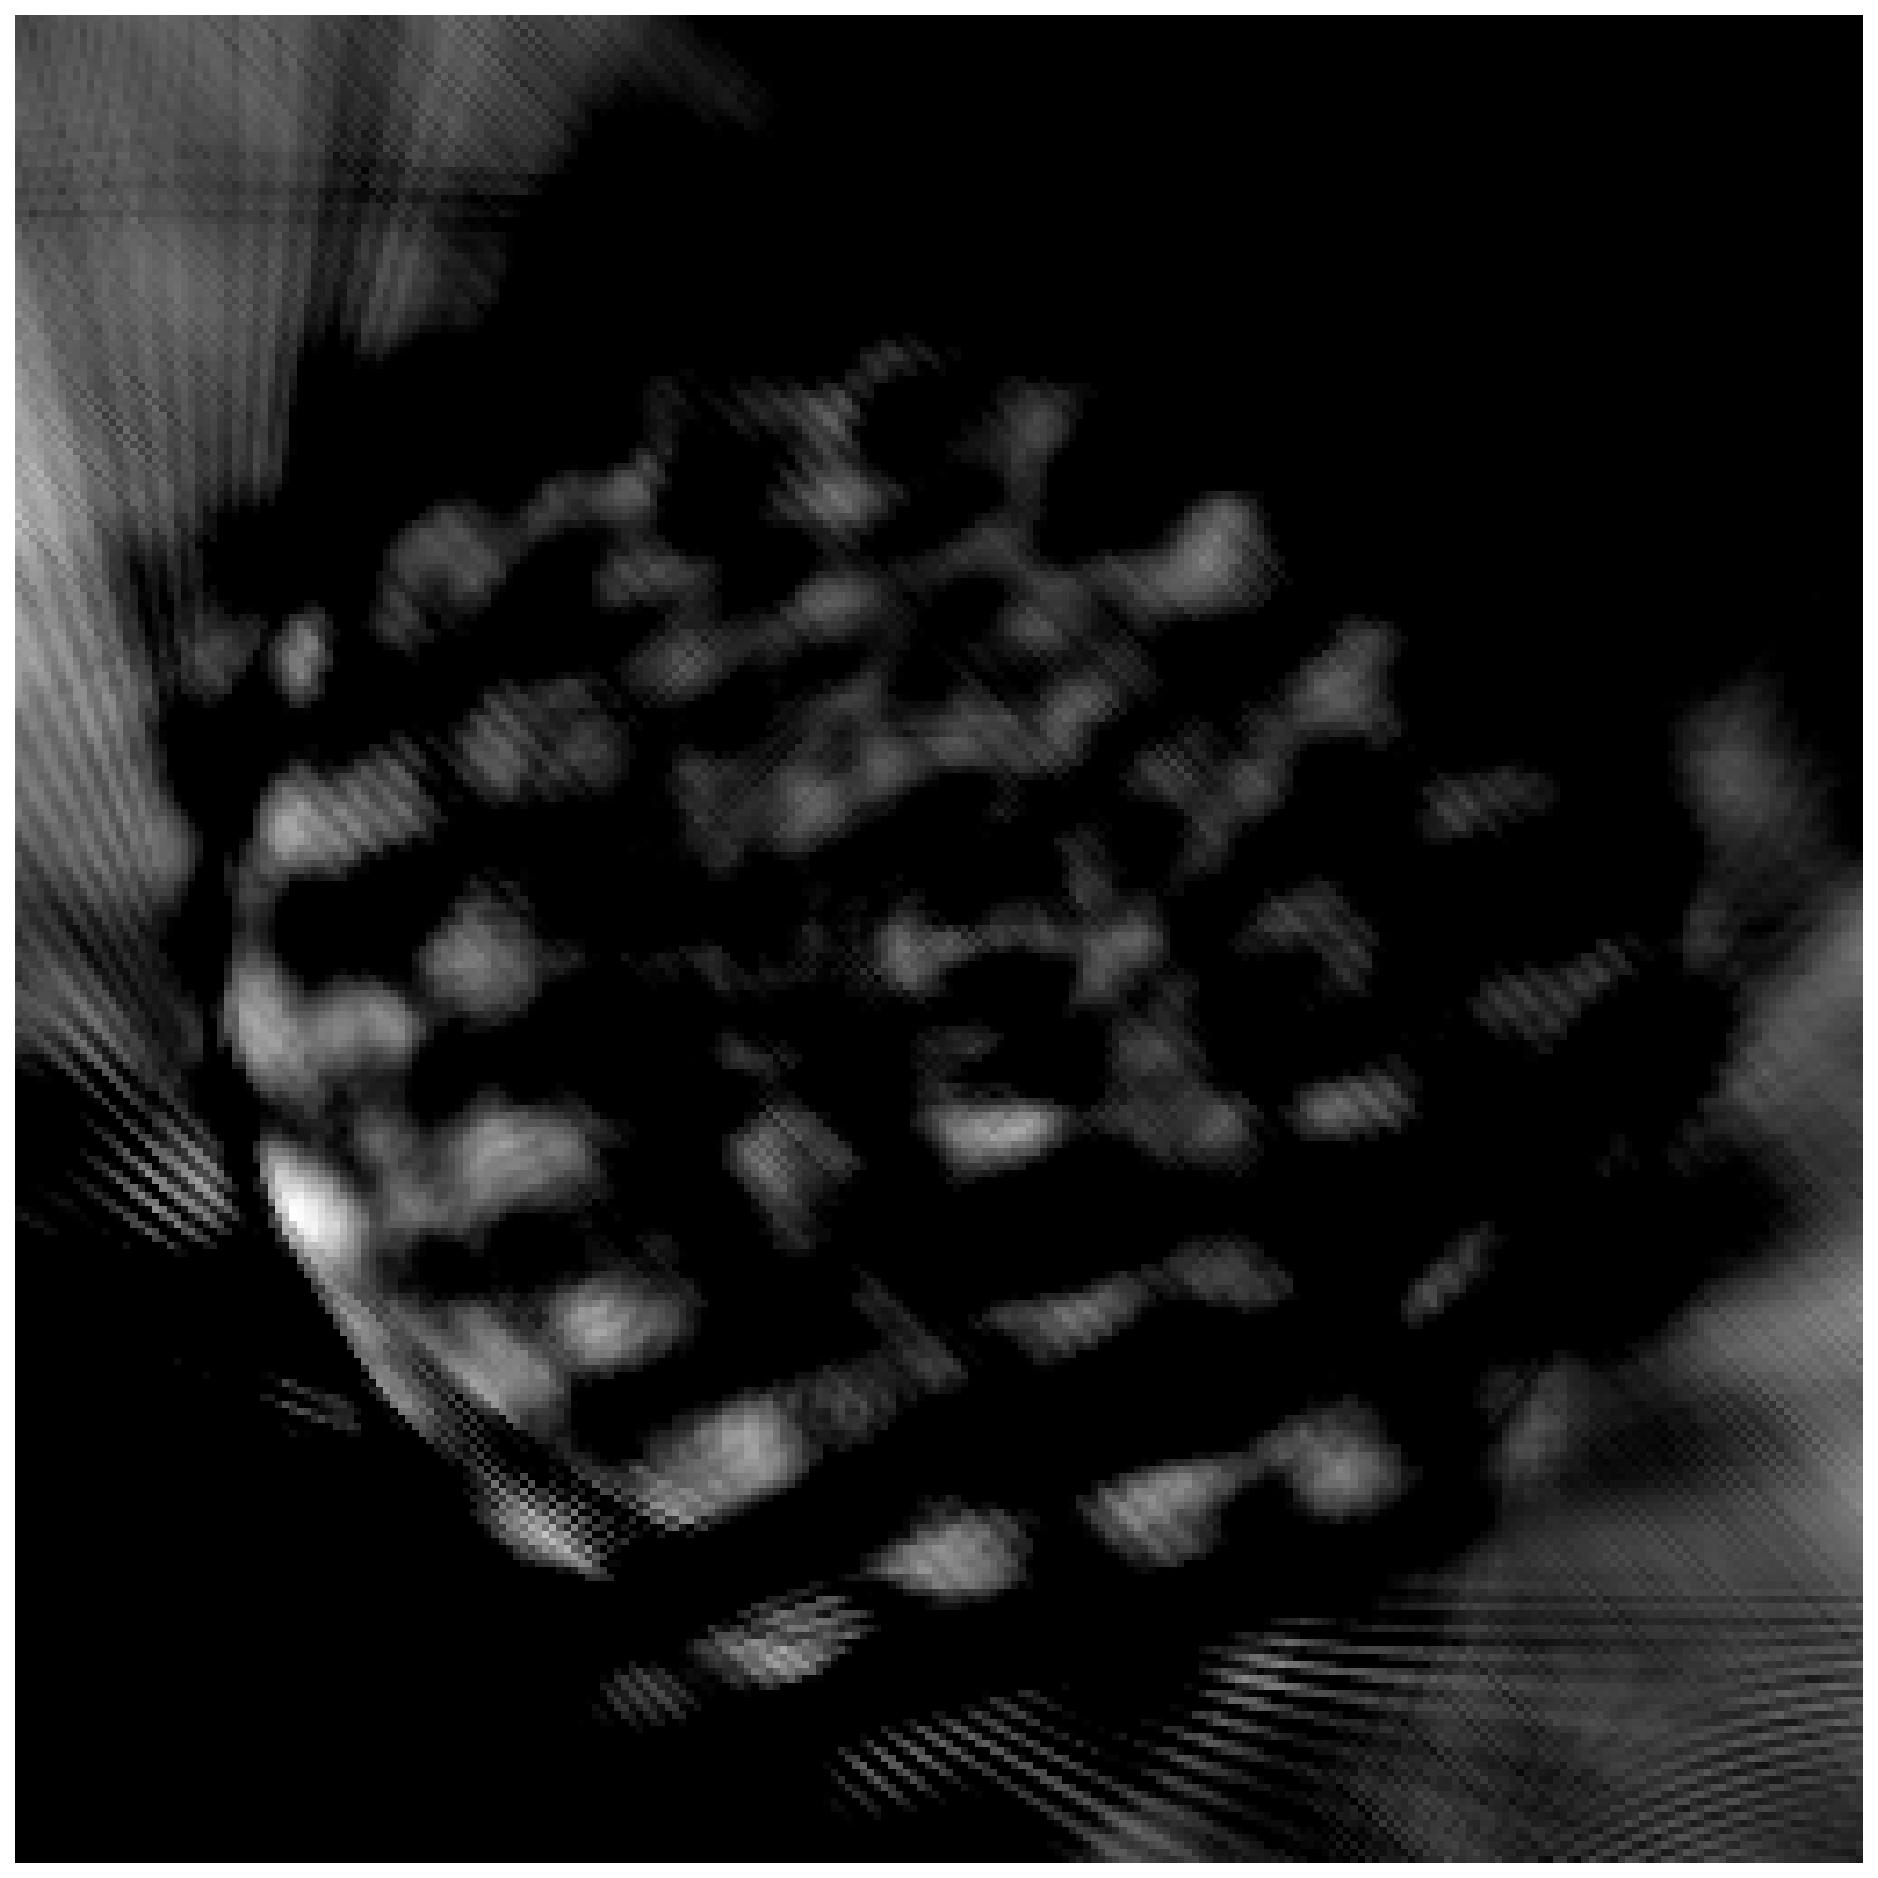
\includegraphics[width=0.2\textwidth]{ reconstructions128_inferenceNoCadUnet.jpg}
\label{fig:reconstructions128_NoCadUnet}}
\hfill
\subfloat[Reconstruction with acquisitions inferred from the Unet with the CAD prior]{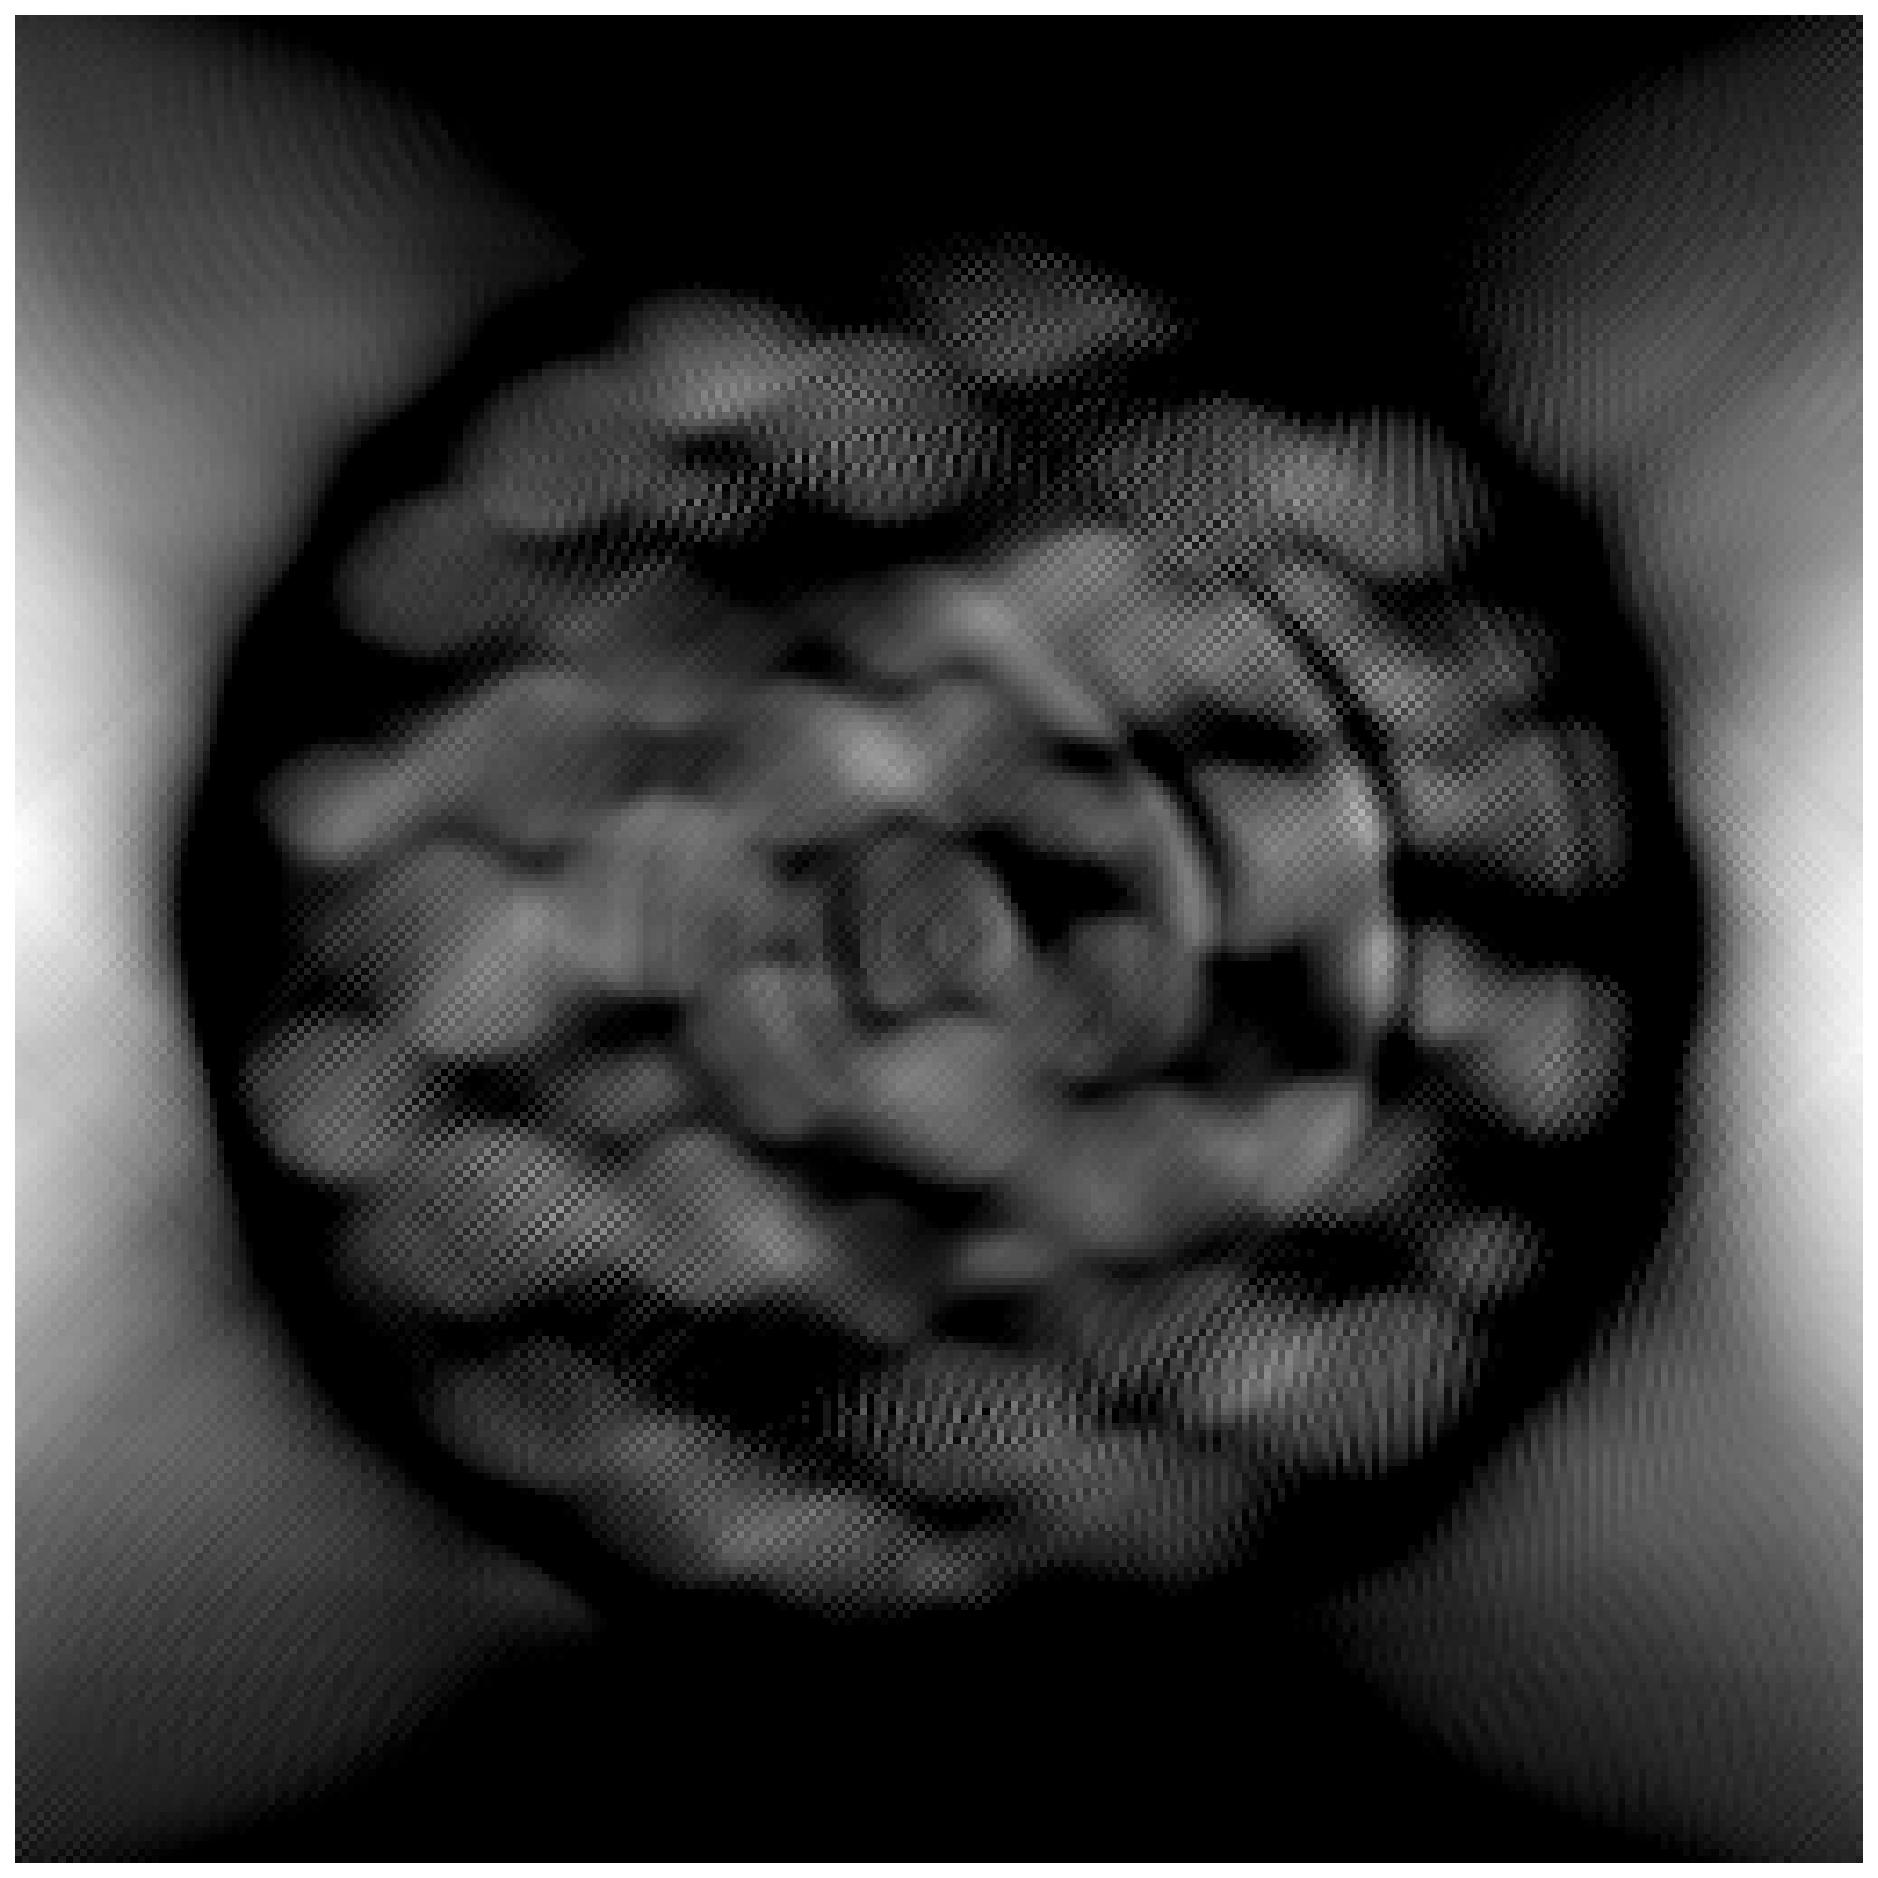
\includegraphics[width=0.2\textwidth]{ reconstructions128_inferenceCadUnet.jpg}
\label{fig:reconstructions128_CadUnet}}
\hfill
\subfloat[Reconstruction with sinogram inpainted by the GAN.]{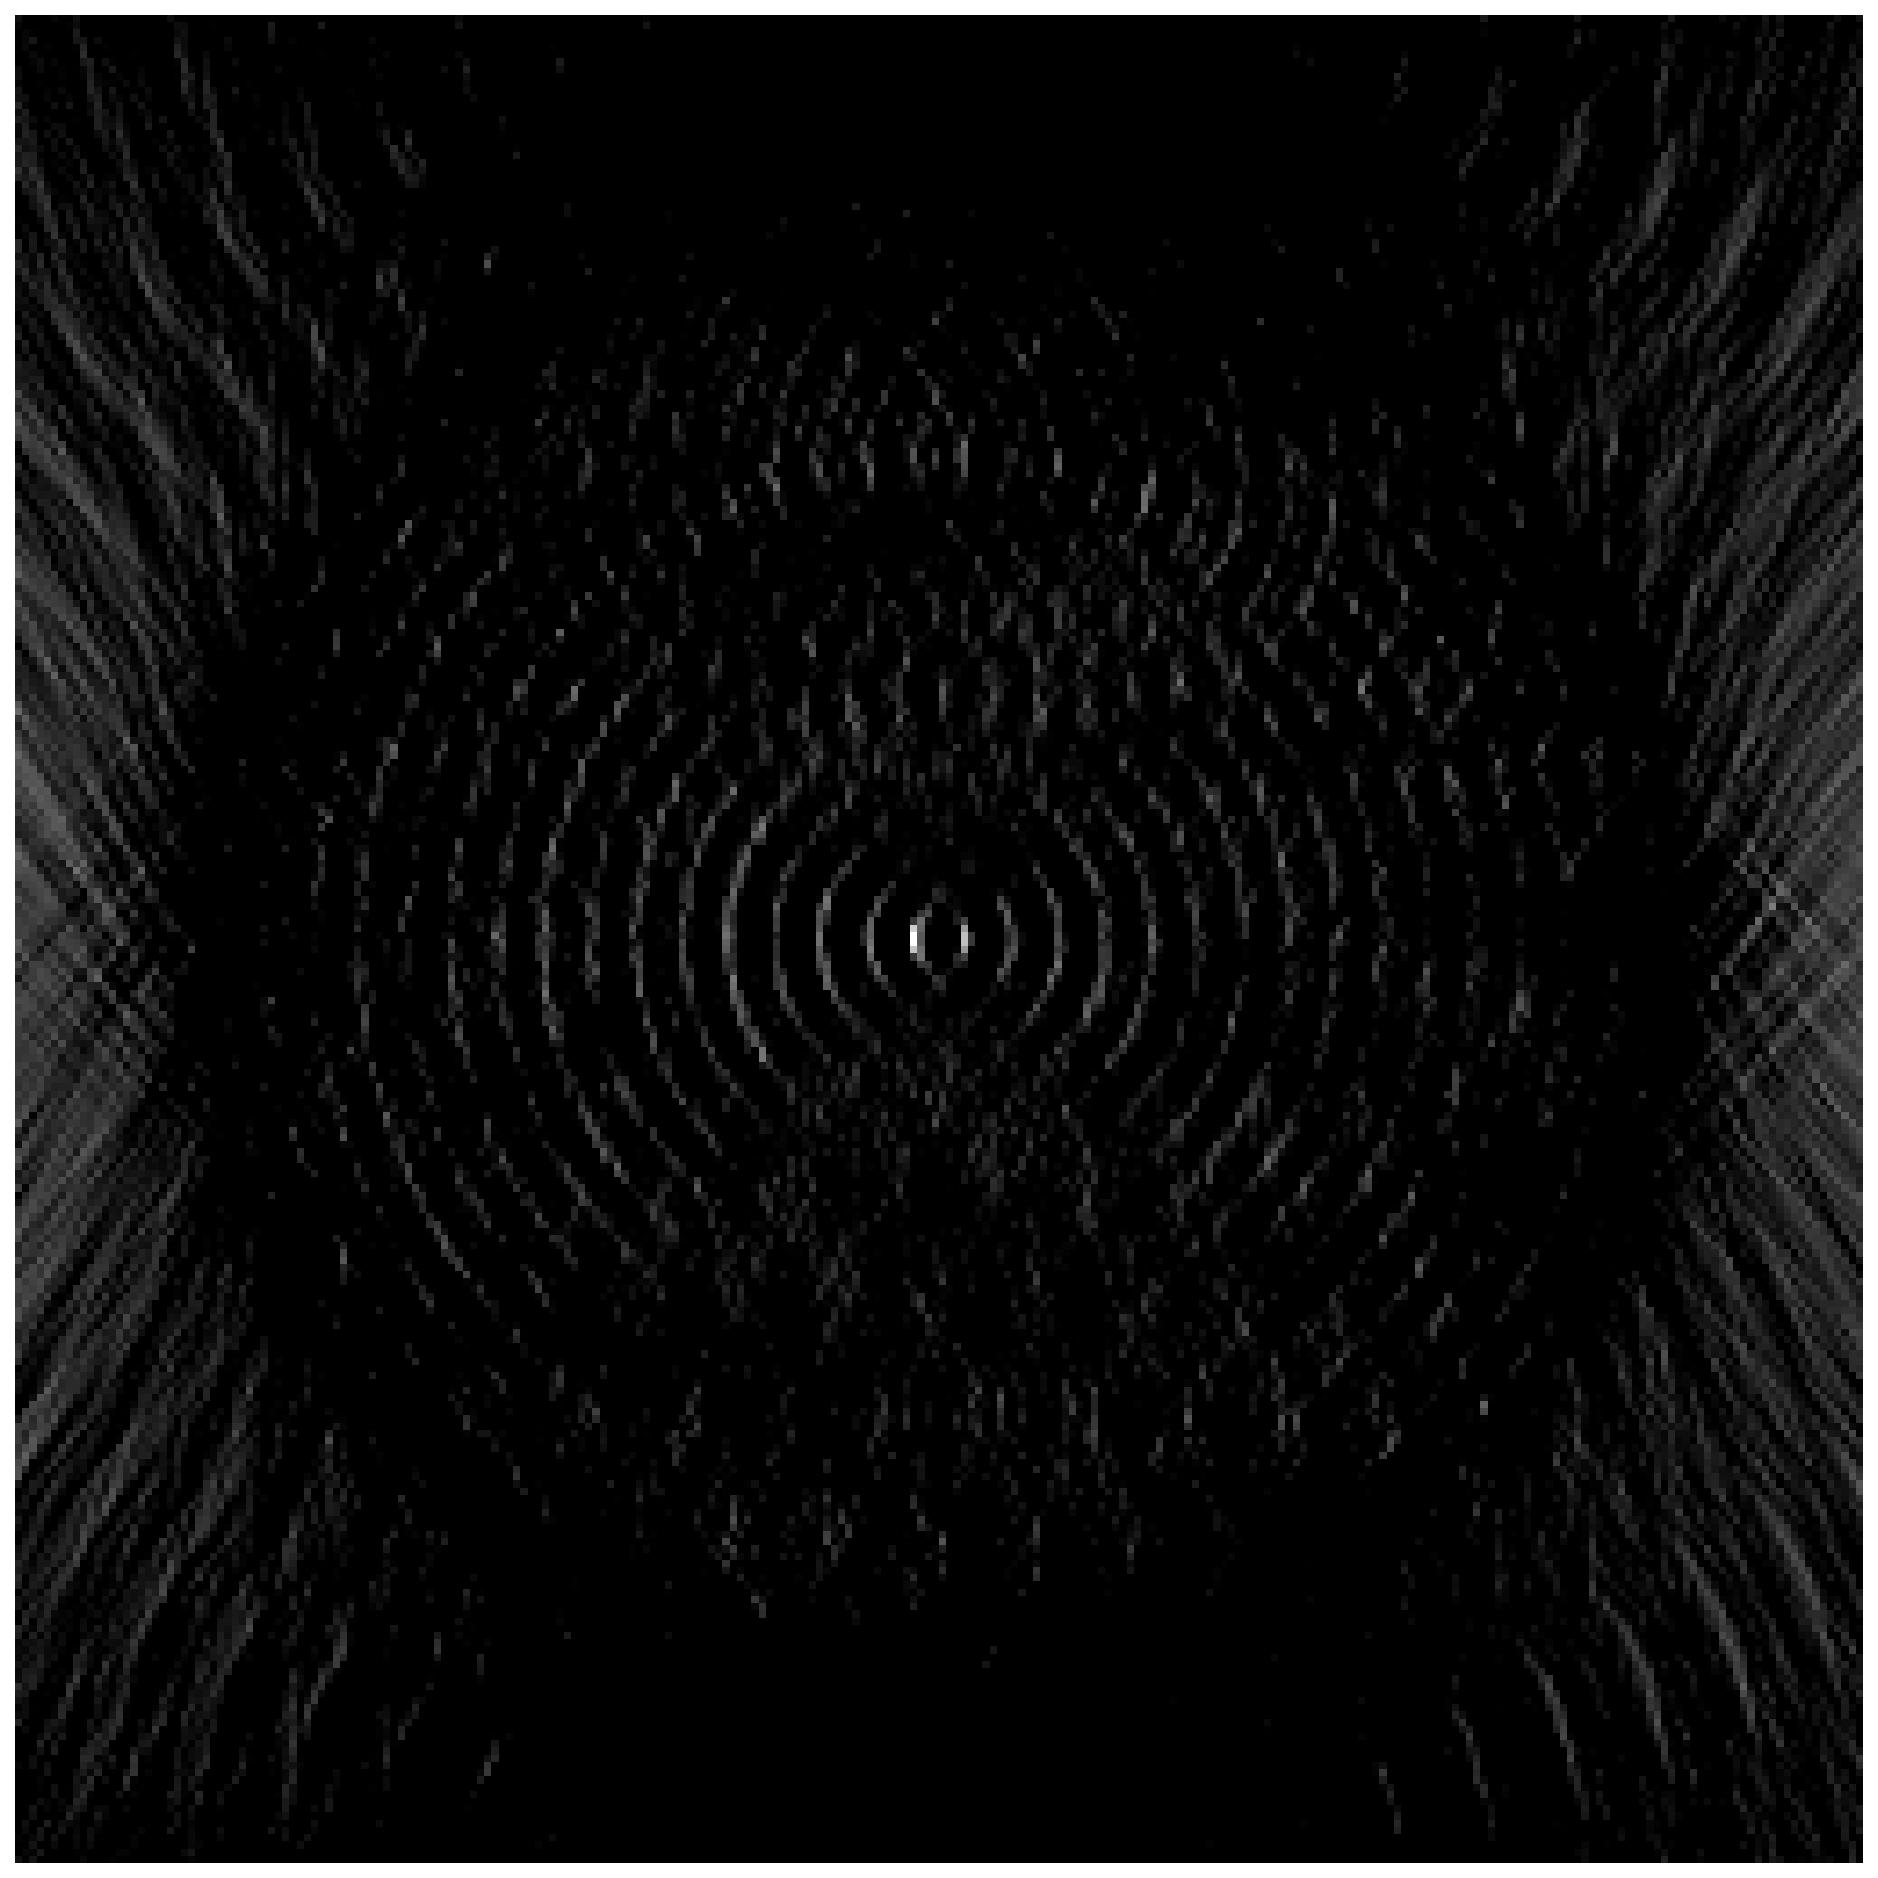
\includegraphics[width=0.2\textwidth]{ reconstructions128_inpaintingNoCadGan.jpg}
\label{fig:reconstructions128_NoCadGan}}
\hfill
\subfloat[Reconstruction with missing acquisitions inferred from the pix2pix architecture using CAD prior.]{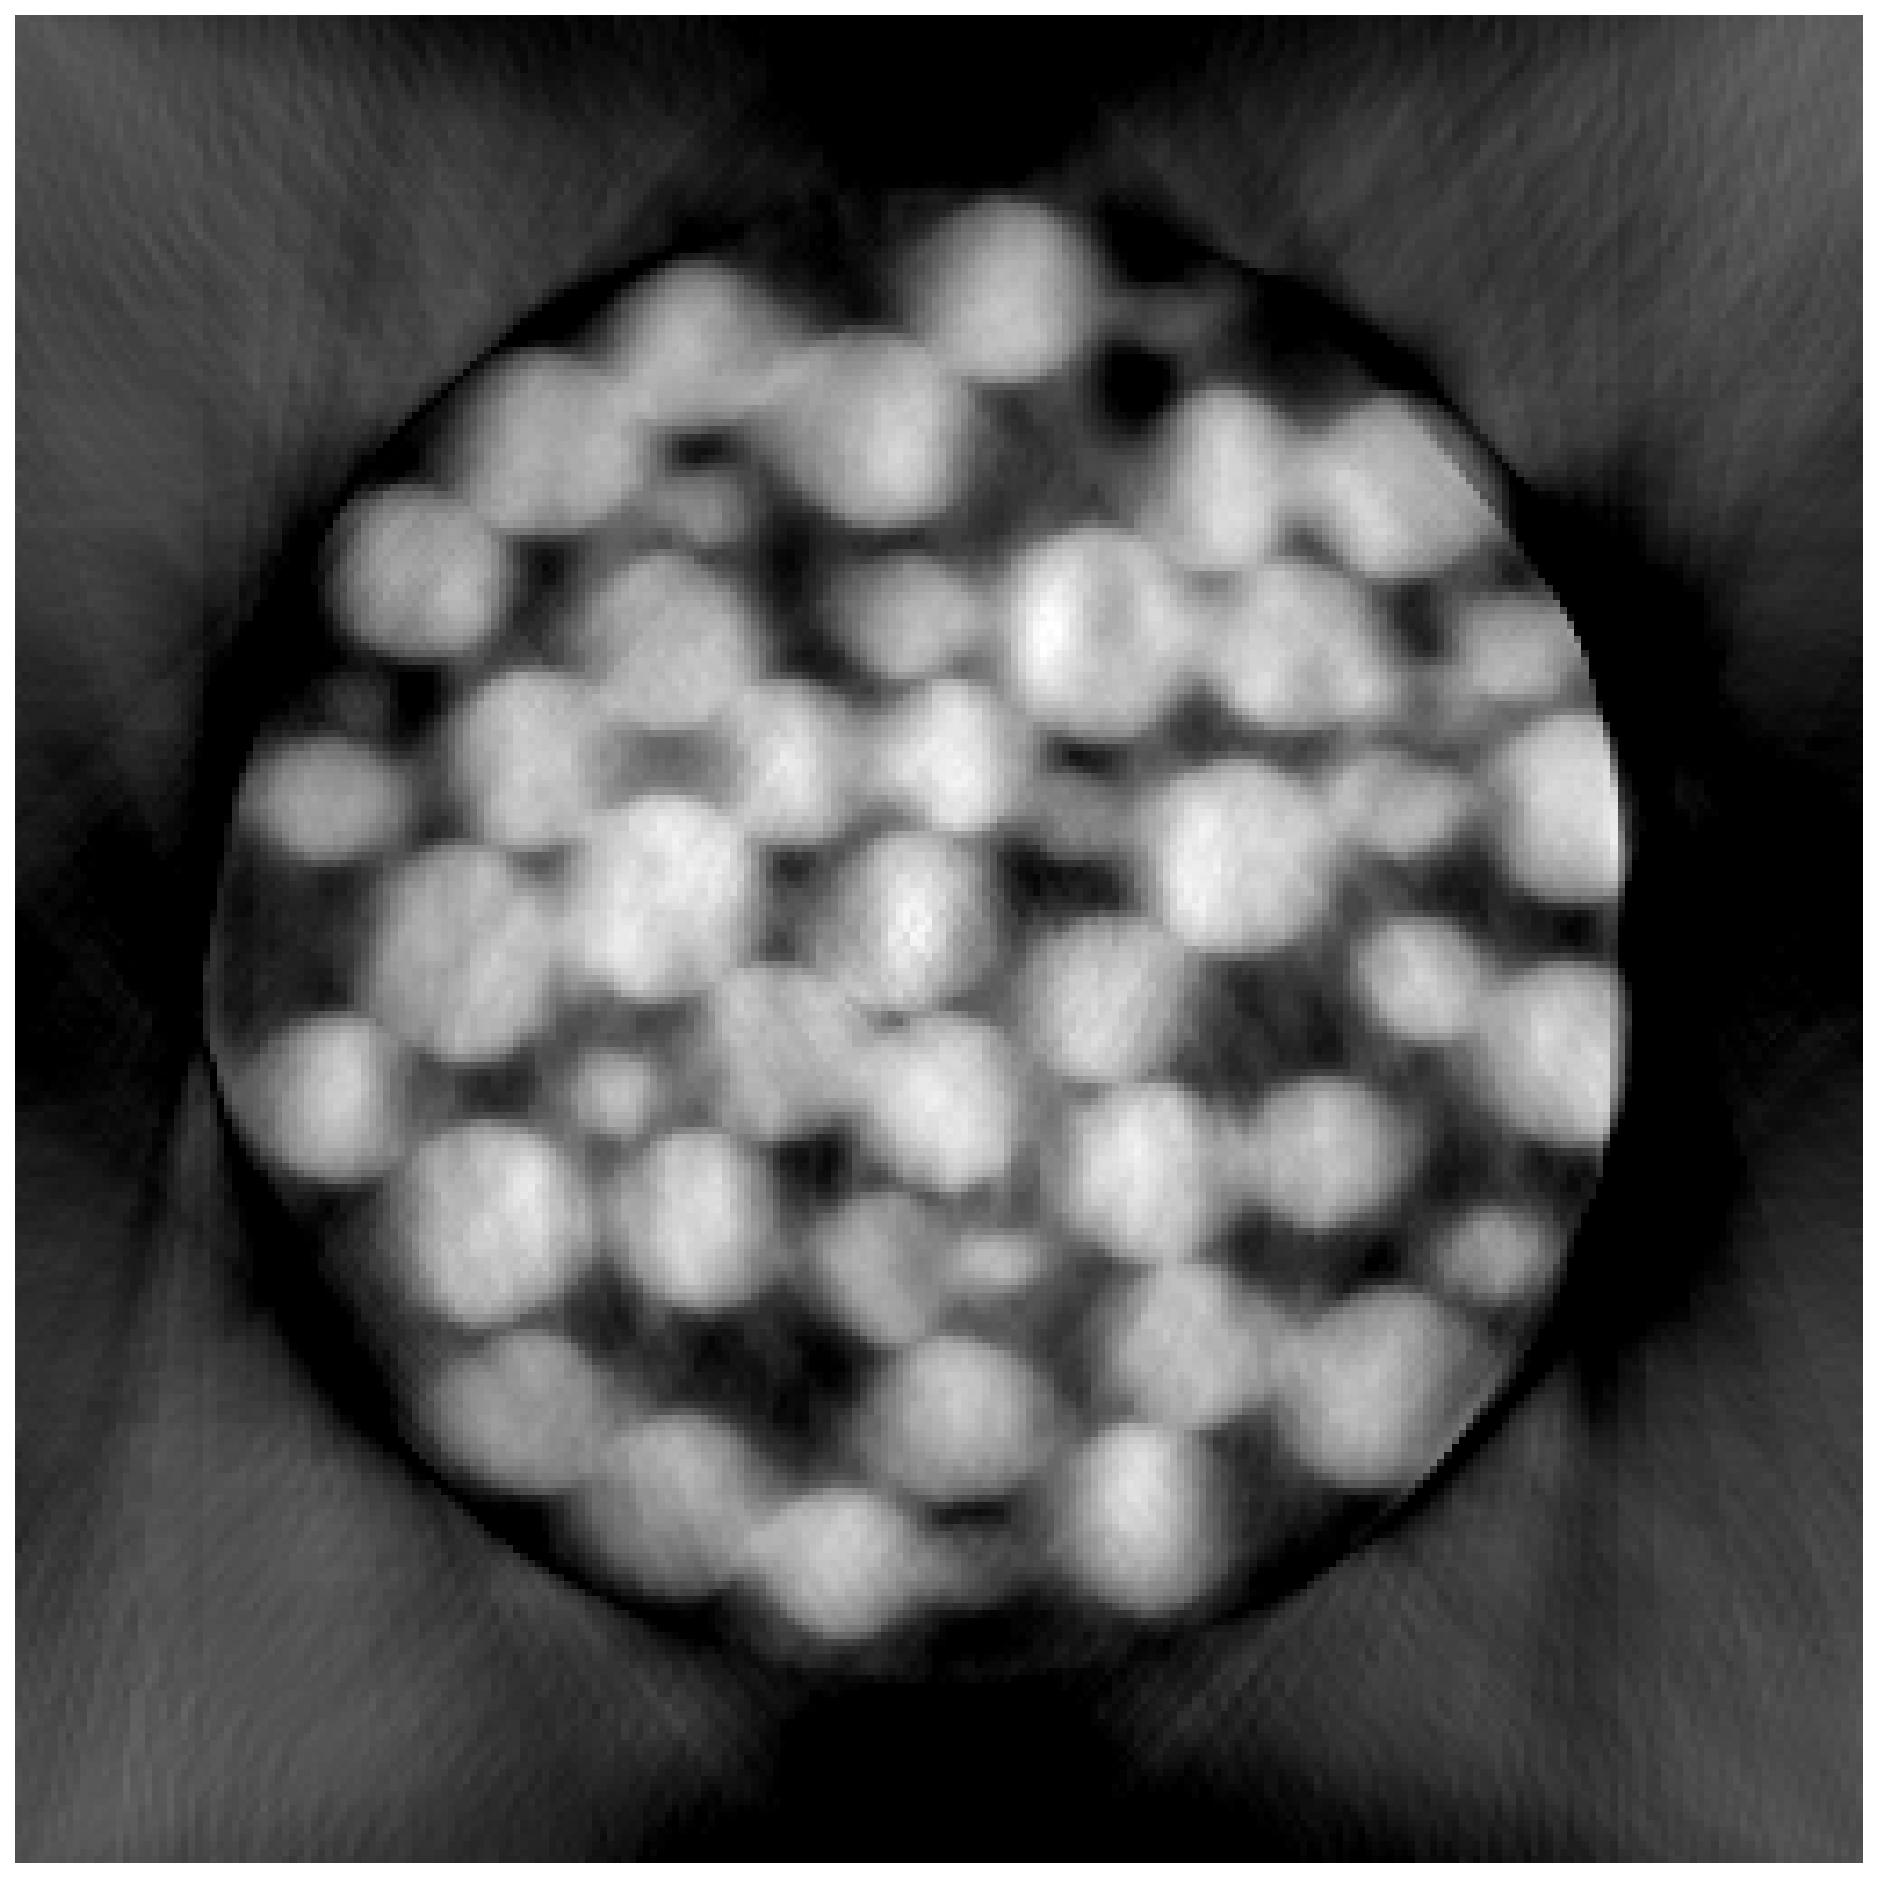
\includegraphics[width=0.2\textwidth]{ reconstructions128_inferenceCadGan.jpg}
\label{fig:reconstructions128_CadGan}}

\label{fig:reconstructions}
\caption{Reconstructions of the first sample of the SophiaBeads test dataset.(\ref{fig:reconstructions128_target}) is the target image, reconstructed from all 256 acquisitions and (\ref{fig:reconstructions128_noInterpolation}) is the image reconstructed from the scarce sinogram. (\ref{fig:reconstructions128_linearInterpolation}) to (\ref{fig:reconstructions128_CadGan}) are the images reconstructed from sinograms enhanced with various methods.}
\end{figure*}  

\end{document}

